\documentclass[10pt,a4paper]{book}
\usepackage[utf8]{inputenc}
\usepackage{amsmath}
\usepackage{amsfonts}
\usepackage{amssymb}
\usepackage{multicol}
\usepackage{hyperref}
\usepackage{tikz}
\usepackage[ruled, lined, longend]{algorithm2e}
\usepackage[shortlabels]{enumitem}
\usepackage{textcomp}

\setlength{\parindent}{20pt}
\hypersetup{
    colorlinks,
    citecolor=black,
    filecolor=black,
    linkcolor=black,
    urlcolor=darkgray
}

\newcommand{\R}{\mathbb{R}}
\newcommand{\N}{\mathbb{N}}
\newcommand{\Z}{\mathbb{Z}}
\newcommand{\F}{\mathbb{F}}
\newcommand{\C}{\mathbb{C}}
\newcommand{\ind}{\hspace*{\parindent}}

\title{Algèbre Linéaire - Notes et Résumés}
\author{Faustine Flicoteaux}
\date{Semestre d'automne 2024}

\begin{document}
\maketitle
\tableofcontents
\newpage


\section*{Introduction}
Ce qui suit est principalement mes propres notes et explications. Évidemment, tout ça ne me vient pas par l'opération du Saint-Esprit, mais du cours de mon professeur, Prof. Jérôme Scherer, et de vidéos et cours en ligne (merci en particulier à 3Blue1Brown).\par 
J'explique principalement des concepts que je ne comprends pas totalement, ce document est donc à prendre avec des pincettes. Si vous remarquez une erreur (mathématique ou de langue), n'hésitez pas à m'en faire part à mon adresse e-mail \texttt{\href{mailto:faustine.flicoteaux@epfl.ch}{faustine.flicoteaux@epfl.ch}}.\par 
Le dernier fichier \LaTeX et le pdf correspondant peuvent être trouvés sur mon dépôt GitHub \url{https://github.com/FocusedFaust/LectureNotes}.

\chapter{Matrices}
\section{Opérations du déterminant}
La multiplication est préservée pour le déterminant, donc $det(A)\cdot det(B) = det(A\cdot B)$. En particulier, $det(A^{-1}) = (det(A))^{-1}$. Par contre, il n'y a pas de formule pour le déterminant d'une addition de matrices, car le déterminant n'est pas linéaire.\par 
Échanger deux lignes ou colonnes revient à multiplier le déterminant par $-1$.\par 
Multiplier une ligne ou une colonne par un scalaire $a$ revient à multiplier le déterminant par ce même scalaire.

\section{Rang d'une matrice, injectivité, surjectivité}
\paragraph{Rang}
Le théorème du rang nous dit que pour une matrice $A$ de taille $m\times n$ ($m$ lignes et $n$ colonnes), $dim(Im(A))+dim(Ker(A))=n$. \par 
Pour une application linéaire $T:V\to W$ et la matrice $B$ représentant cet transformation, on a que $dim(Im(A))+dim(Ker(A))=dim(V)$.
\paragraph{Injectivité}
Une matrice est injective si sa forme échelonnée-réduite a un pivot dans chaque colonne.
\paragraph{Surjectivité} 
Une matrice est surjective si sa forme échelonnée-réduite a un pivot dans chaque ligne.

\section{Valeurs propres facilement repérables}
Certaines valeurs propres peuvent être facilement repérables, sans avoir à passer par le polynôme caractéristique, ce qui nous évite de perdre pas mal de temps quand on a des grandes matrices. \par 
Il est utile de noter que pour une matrice $A$ diagonalisable, $A^T$ a les mêmes valeurs propres.
\begin{itemize}
\item Si deux colonnes (ou plus) sont linéairement dépendantes, alors le $Ker$ de la matrice n'est pas nul et 0 est une valeur propre (et donc la matrice $A$ n'est pas inversible car son déterminant vaut 0). 
\item Les matrices triangulaires (supérieures ou inférieures) on comme valeurs propres les coefficients placés dans la diagonale.
\item Si une des colonnes est vide sauf en $a_{ii}$ avec $i$ l'index de la colonne, alors le coefficient $(a_{ii})$ est une valeur propre. En effet, si on calcule $A-(a_{ii})\cdot I_n$, on se retrouve avec une colonne nulle. On a donc forcément $dim(Ker(A)) > 0$ et donc $(a_{ii})$ est une valeur propre. 
\item Si la somme des coefficients des lignes est la même pour toutes les lignes ou si la somme des coefficients des colonnes est la même pour toutes les colonnes, alors cette somme est valeur propre de la matrice (prouvé en exercice).
\item Si $A$ est diagonalisable, alors la trace de $A$ est égale à la somme des valeurs propres de $A$. Ainsi, si il nous manque une seule valeur propre (attention à la multiplicité), on peut la calculer à partir de la trace.
\end{itemize}

\section{Factorisation \texorpdfstring{$QR$}{QR}}
Le but de la factorisation $QR$ est de trouver une décomposition d'une matrice $A$ telle que $Q\cdot R=A$ avec la matrice $Q$ qui soit orthogonale et la matrice $R$ qui soit triangulaire supérieure.\par 
Pour trouver la matrice $Q$, on utilise la méthode de Gram-Schmidt sur les colonnes de $A$, pour en obtenir une base orthogonale de l'espace-colonne. On divise ensuite les vecteurs obtenus pour les normaliser.\par 
La matrice $R$ correspond aux colonnes de $A$ exprimés dans la base de $Q$. Puisque $Q\cdot R=A$ et que $Q$ est orthonormée ($Q^{-1}=Q^T$), on peut alors calculer $R=Q^T\cdot Q\cdot R=Q^T\cdot A$. \par
Sinon, on peut remarquer que la matrice $R$ correspond à l'inverse (donc signe inverse) des opérations élémentaires effectuées lors du "Gram-Schmidt-age" de $A$. On multiplie ensuite chaque ligne de $R$ ainsi obtenu par la norme des vecteurs de $Q$ avant normalisation (méthode certes plus rapide mais plus prône aux erreurs).\par 
Additionnellement, une manière de trouver un coefficient particulier de $R$, on calcule $r_{ij} = q_i\cdot a_j$.

\section{Théorème et décomposition spectrale}
Si une matrice est symétrique, il découle plusieurs propriétés. Premièrement, son inverse (et la transposée) sont aussi symétriques. Deuxièmement, cette matrice est orthodiagonalisable. Ceci veut dire qu'il existe une base \textbf{orthogonale} de ses vecteurs propres.\par 
Pour orthodiagonaliser une matrice symétrique, on la diagonalise comme habituellement, puis on vérifie que ses vecteurs propres sont bien orthogonaux. Si ils ne le sont pas, on les orthogonalise grâce au procédé de Gram-Schmidt.\par 
La matrice $P$ dont les colonnes sont les vecteur propres orthogonaux est une matrice orthogonale. $P^TAP$ est donc diagonale ($P^{-1}=P^T$).
\paragraph{Décomposition spectrale} 
Soit $A$ symétrique, $U$ orthogonale et $U^TAU=D$ diagonale. Le \textbf{spectre} est l'ensemble des valeurs propres de $A$. La décomposition spectrale de $A$ est
\[A=\lambda_1\overrightarrow{u_1}\overrightarrow{u_1}^T+\ldots+\lambda_n\overrightarrow{u_n}\overrightarrow{u_n}^T\]

\chapter{Bases et matrices}

\section{Représentation dans une base}
Soient un espace vectoriel $V$, un vecteur $\vec{v} = \begin{pmatrix} v_1 \\ \vdots \\ v_n \end{pmatrix}$ et une base $\mathcal{B}$ de $V$. Pour trouver les coordonnées de $\vec{v}$ dans la base $\mathcal{B}$, il faut résoudre le système $B\vec{x} = \vec{v}$ avec $B$ la matrice qui représente la base $\mathcal{B}$ et $\vec{x} = \begin{pmatrix} x_1 \\ \vdots \\ x_n \end{pmatrix} = (\vec{v})_\mathcal{B}$, c'est à dire le vecteur $\vec{v}$ exprimé selon la base $\mathcal{B}$.

\section{Changements de bases}
Soit V un espace vectoriel. On peut représenter un vecteur de cet espace en fonction d'une base arbitraire. Lorsqu'on change de base, la représentation sera alors différente. C'est-à-dire qu'un vecteur $\vec{b}$ n'a pas les mêmes coordonnées en fonction de la base dans laquelle il est représenté. \par 
Soit une base $\mathcal{B}=(\vec{b_1}, \vec{b_2})$. Un vecteur $(x)_{\mathcal{B}}=(x_1,x_2)$ signifie $x_1\cdot \vec{b_1}+x_2\cdot \vec{b_2}$. Pour trouver les valeurs qu'auraient $x_1$ et $x_2$ dans une autre base, par exemple $\mathcal{C}=(\vec{c_1}, \vec{c_2})$ on utilise une matrice de changement de base, selon l'égalité suivante: 
\[(Id)^{\mathcal{C}}_{\mathcal{B}} (x)_{\mathcal{B}} = (x)_{\mathcal{C}}\]
La matrice $(Id)^{\mathcal{C}}_{\mathcal{B}}$ est la matrice de changement de base de $\mathcal{B}$ vers $\mathcal{C}$. Comme dit Prof. Scherer : "\textit{Elle mange des vecteurs en base $\mathcal{B}$ pour donner des vecteurs en base $\mathcal{C}$}". \par 
Pour la trouver, on écrit la matrice augmentée $[\vec{c_1},\vec{c_2}\ |\ \vec{b_1},\vec{b_2}]$ puis on l'échelonne et la réduit. Cela permet d'exprimer les coordonnées des vecteurs de la base $\mathcal{B}$ comme combinaison linéaire des vecteurs de la base $\mathcal{C}$, c'est-à-dire que $(Id)^{\mathcal{C}}_{\mathcal{B}} = ((\vec{b_1})_{\mathcal{C}},(\vec{b_2})_{\mathcal{C}})$.\par 
On remarque alors que la matrice de changement de base est une transformation linéaire (et même un endomorphisme) qui permet de projeter les vecteurs d'une base sur les vecteurs d'une autre base. Tout vecteur autre sera alors projeté sur sa représentation en une autre base. C'est-à-dire qu'un vecteur $(a,b)_\mathcal{C}$ sera projeté sur $(a,b)_\mathcal{B}$ (mêmes coordonnées mais vecteurs différents) alors qu'un vecteur $(a,b)_\mathcal{B}$ sera projeté sur $(c,d)_\mathcal{C}$(même vecteur mais différentes coordonnées). 

\paragraph{Changement de base inverse}
Puisque le changement de base peut s'appa\-renter à une transformation linéaire, le changement inverse est la transformation linéaire inverse. $(Id)^{\mathcal{B}}_{\mathcal{C}} = ((Id)^{\mathcal{C}}_{\mathcal{B}})^{-1}$

\paragraph{Astuce}
Il y a un moyen plus rapide de calculer une matrice de changement de base : $(\vec{c_1},\vec{c_2})^{-1}\cdot (\vec{b_1},\vec{b_2}) = (Id)^{\mathcal{C}}_{\mathcal{B}}$\footnote{\textit{Cette méthode n'a pas été démontrée par le prof (et encore moins par moi), c'est donc à utiliser à vos risques et périls.}}

\paragraph{Cas de la base canonique}
La base canonique se note $\mathcal{C}an = (e_1,...,e_n)$ avec $e_i$ des vecteurs dont les coordonnées valent 0 sauf quand l'index est égal à $i$, ou elle vaut 1. C'est la base la plus "naturelle" pour nous autres, pauvres mortels, pour se représenter un espace vectoriel. La matrice de changement de base est alors assez intuitive : $(Id)^{\mathcal{C}an}_{\mathcal{B}}$ est la matrice ayant pour colonnes les vecteurs de la base $\mathcal{B}$.

\paragraph{Astuce en examen}
Pour une question à choix multiples de type "\textit{Soit deux bases données, quelle est la matrice de changement de base ?}" il n'est pas forcément utile de calculer la matrice entière. Il ne faut pas non plus commencer par le premier vecteur. Il est plus rapide de trouver pour les matrice proposée une colonne qui est différente pour chaque proposition. Ensuite, on peut calculer $(\vec{b_i})_\mathcal{C}$ correspondant.\par 
Le temps est compté en examen. Il faut donc essayer d'éliminer le plus de réponses possibles en le moins de calculs possibles.

\section{Matrice d'une application selon une base}
Il peut être demandé de construire la matrice d'une application linéaire $T$ mais dans une base spécifique, disons $\mathcal{B}=(\vec{b_1},...,\vec{b_n})$. Dans ce cas la matrice sera $M = [(T(\vec{b_1}))_\mathcal{B}\ ...\ (T(\vec{b_n}))_\mathcal{B}]$.

\paragraph{Astuce en examen}
Lors du calcul de la matrice d'une transformation selon une base, il faut bien penser à exprimer le résultat de chaque $T(\vec{b_i})$ selon la base demandée.

\section{Matrice d'une transformation linéaire}
Soit $T:V\to W$ une transformation linéaire de $V$ vers $W$. Pour construire la matrice représentant cette transformation, on choisit une base de $V$ et une base de $W$ (habituellement des bases canoniques). Les colonnes de la matrice $A$ de $T$ sont les images des vecteurs de la base de $V$ exprimés dans la base de $W$. \par 
On voit dans le cas d'un endomorphisme ($T:V_\mathcal{B}\to V_\mathcal{C}$) ou l'on choisit deux bases $\mathcal{B}$ et $\mathcal{C}$ différentes pour $V$, que la matrice sera les vecteurs de $\mathcal{B}$ dans la base $\mathcal{C}$.

\chapter{Corps finis}
\paragraph{Caractéristique et cardinalité}
La caractéristique d'un corps fini $K$ est le plus petit entier non nul $n$ tel que $n\cdot 1_K = 0$. On le note $carK$. Cette caractéristique est un nombre premier.\par 
Soit $K$ un corps fini et $p=carK$. Alors il existe $n$ tel que $K$ a $p^n$ éléments. Ce nombre est la cardinalité de $K$.

\section{Corps à partir de nombres premiers} \label{Visualisation}
Les corps finis avec un nombre premier d'élément sont de prime abord relativement simples (je dis relativement parce qu'on fait quand même de la théorie des corps). Un corps $\F_p$ est un corps à $p$ éléments $\{0,1,...,p-1\}$. Toutes les opérations se font \textit{modulo} $p$, c'est à dire qu'on ne considère que le reste de la division entière par $p$.\par 

\paragraph{Opposé}
Chaque nombre $x\neq 0$ admet un opposé $-x$ tel que $x+(-x)=0$.\par
Par exemple, dans le corps $\F_7$, l'opposé de 3 est 4 car $3+4=7=0$.

\paragraph{Inverse}
Chaque nombre $x\neq 0$ admet un inverse $x^{-1}$ tel que $x\cdot x^{-1}=1$.\par
Par exemple, dans le corps $\F_7$, l'inverse de 3 est 5 car $3\cdot 5=15=1$.

\paragraph{}
Je visualise les nombres réels comme une droite horizontale, faite d'une infinité de points et donc de valeurs. Par extension, les nombres complexes sont un plan, puisqu'ils sont constitués de deux réels (la partie réelle et la partie imaginaire)(mais c'est un sujet pour une autre fois). \par
Par contre, je vois les corps finis comme un segment de longueur $p-1$ et ayant un point toutes les unités, qui représente un élément de ce corps. Puisque toutes les opérations se font \textit{modulo p}, un calcul qui se "promène" le long du segment, revient au début lorsqu'il dépasse la valeur $p-1$. C'est comme les effets spéciaux dans les films, quand un personnage passe la tête dans une porte et que sa tête ressort d'une autre porte du même couloir.

\section{Corps à partir de polynômes}
Lorsque l'on veut former un corps dont le nombre d'éléments n'est pas premier, on se rend compte que l'addition et la multiplication ne permettent pas d'en faire un groupe abélien. Pour former un corps, au lieu des entiers, on utilise des polynômes $\F_p[t]$ comme éléments et la division euclidienne est remplacée par la division polynomiale.\par 
Pour former un corps, il nous faut un polynôme $p(t)$ unitaire irréductible de degré $n$ dans $\F_p[t]$. Ensuite, on considère l'ensemble de tous les restes de division par $p(t)$. Il y en a $p^n$.

\subsection{Trouver des polynômes irréductibles}
Lors de la construction d'un corps fini, il nous est parfois explicitement demandé de trouver un polynôme irréductible. Pour cela, il y a plusieurs méthodes. 
\begin{enumerate}
\item Énumérer les polynômes non-constants de degré inférieur à celui voulu et diviser tous les polynômes de degré voulu par ceux-ci. Cela peut être laborieux, surtout pour les degrés élevés.
\item Tester les racines possibles. Cela est particulièrement efficace pour les coefficients dans $\F_p$ avec $p$ relativement petit. 
\item Il y a également une méthode reposant sur la divisibilité de $x^{p^n}-x$, mais je ne la connais pas assez. Si cela vous intéresse, je vous conseille d'aller chercher du côté de la "condition de divisibilité"\footnote{En gros (très gros même), $p(x)$ est irréductible dans $\F_{p^n}$ si il divise $x^{p^n}-x$, mais pas $x^{p^k}-x\ \forall k<n$.}.
\end{enumerate}

\section{Linéarité et distributivité modulaire}
L'opération "modulo" n'est absolument pas linéaire. Cependant, il existe une certaine distributivité de l'arithmétique modulaire.
\[(a+b)\ mod\ n = ((a\ mod\ n)+(b\ mod\ n))\ mod\ n\]
\[(a-b)\ mod\ n = ((a\ mod\ n)-(b\ mod\ n))\ mod\ n\]
\[(a\cdot b)\ mod\ n = ((a\ mod\ n)\cdot(b\ mod\ n))\ mod\ n\]
\paragraph{Preuve}
On prouve la distributivité de la soustraction ainsi, pour les curieux.\par 
Soit:
\[a \mod n = r_1 \quad \text{et} \quad b \mod n = r_2,\text{ où :}\]
\[a = k_1 n + r_1 \quad \text{et} \quad b = k_2 n + r_2,\]
pour \(k_1,k_2\in\N\), et \(0 \leq r_1, r_2 < n\).
La différence \(a - b\) est :
\[a - b = (k_1 n + r_1) - (k_2 n + r_2) = (k_1 - k_2)n + (r_1 - r_2).\]
En prenant le module \(n\), il nous reste :
\[(a - b) \mod n = (r_1 - r_2) \mod n.\]
D'un autre côté, on considère l'expression :
\[\big((a \mod n) - (b \mod n)\big) \mod n.\]
En substituant \(a \mod n = r_1\) et \(b \mod n = r_2\), on a :
\[\big((a \mod n) - (b \mod n)\big) \mod n = (r_1 - r_2) \mod n.\]
Ainsi,
\[(a - b) \mod n = \big((a \mod n) - (b \mod n)\big) \mod n.\]

\chapter{Astuces et reminders pour l'examen}
\section{Est-ce un sous-espace vectoriel ?}
Pour montrer si un ensemble est un sous-espace vectoriel, il faut prouver que
\begin{enumerate}
\item l'addition de deux éléments appartient toujours à l'ensemble
\item un élément multiplié par un scalaire reste dans l'ensemble
\end{enumerate}
Particulièrement, il faut que l'élément nul (i.e. $\overrightarrow{0}, p(x)=0,$ ...) appartienne à l'ensemble. Si il n'y est pas, c'est éliminatoire. Ensuite, on vérifie les deux points mentionnés, selon l'ensemble en question.\par 
Par exemple, pour un ensemble $W^\bot$ orthogonal au sous-espace vectoriel $W$ de $R^n$. 
\begin{enumerate}
\item Soit $x,y\in W^\bot$ et $w\in W$. $(x+y)\cdot w=x\cdot w+y\cdot w=0+0=0$, ce qui démontre le point 1 ci-dessus.
\item Soit $\alpha\in\R$ et $x\in W^\bot$. Alors $(\alpha x)\cdot w=\alpha(x\cdot w)=\alpha0=0$.
\end{enumerate}

\section{Calcul de l'inverse d'une matrice}
Cette méthode m'a été transmise par mon incroyable professeur de l'année dernière, M. Ischi, et s'est avérée très utile. Elle marche principalement sur les matrices $2\times 2$ et $3\times 3$ (au-delà, les calculs ne sont pas plus simples que la formule "officielle"). Pour une matrice $A$, on calcule les coefficients de son inverse tels que 
\[(a^{-1})_{ij} = \dfrac{1}{detA} det((A^T)_{ij})\]
où $(A^T)_{ij}$ est la matrice transposée à laquelle on a enlevé la ligne $i$ et la colonne $j$. C'est-à-dire que chaque coefficient de la matrice inverse est le déterminant de $(A^T)_{ij}$, divisé par le déterminant de $A$. Attention cependant, parce que chaque coefficient est multiplié par un signe selon sa ligne et sa colonne, comme suit :
\[\begin{pmatrix}
 + & - & +\\
 - & + & -\\
 + & - & +
\end{pmatrix}\]
Attention, Il faut bien utiliser la transposée de la matrice à inverser, et non la matrice elle-même.

\section{Contres-exemples courants}
Il est utile de tester les propositions données avec des contres exemples typiques. Pour les matrices, on a :
\begin{itemize}
\item $\big(\begin{smallmatrix} 
1 & 0\\
0 & 0
\end{smallmatrix}\big)$, 
$\big(\begin{smallmatrix} 
0 & 1\\
0 & 0
\end{smallmatrix}\big)$, 
$\big(\begin{smallmatrix} 
0 & 0\\
1 & 0
\end{smallmatrix}\big)$ et  
$\big(\begin{smallmatrix} 
0 & 0\\
0 & 1
\end{smallmatrix}\big)$, notamment pour l'inversibilité.
\item La matrice identité
\item La matrice nulle
\item Une matrice qui ne soit pas carrée (pour l'inversibilité). Effectivement, il ne faut pas supposer qu'une matrice soit inversible, à moins que ça ne soit explicitement dit dans l'énoncé.
\end{itemize}
Il arrive parfois dans les vrais/faux qu'on nous présente une proposition contenant des $\alpha_i$, des réels arbitraires. Attention, car ces réels peuvent être 0. L'indépendance linéaire ne tient plus.

\section{Erreurs de nomenclature}
Attention, orthonormé $\neq$ orthogonal. Dans les questions portant sur des bases orthonormées, il faut veiller à éliminer d'office les bases qui ne le sont pas.\par 
Ce n'est pas une \textbf{unique} solution si la solution est un sous-espace vectoriel.

\appendix
\chapter{Corps finis complexes}
Je me suis posé la question à un moment dans mes révisions : "Peut-on construire un corps fini complexe, c'est-à-dire un corps $\C_p$ qui soit tous les nombres complexes ayant des coefficients dans $\F_p$ ?". J'ai posé la question à Yacine (ce crack en analyse) et on a étudié la possibilité. \par 
Il faudrait pour cela que chaque nombre $\neq 0$ ait un opposé et un inverse. Pour les opposés, ça semble plutôt simple puisque $-ai = pi-ai = (p-a)i$ et donc, par extension, $-(a+ib)=-a-ib=(p-a)+(p-b)i$.\par 
Pour les inverses cependant, la situation est plus délicate. L'inverse d'un complexe se définit comme
\[z^{-1}=\frac{a-ib}{a^2+b^2}\]
On a alors souvent des fractions comme coefficients. Cependant, ce n'est pas un problème car $1/n = n^{-1}$, c'est donc l'inverse de $n$, qui doit exister dans $\F_p$ aussi (si $n\neq 0$, on y vient). Donc si $n\neq 0$, on utilise son inverse. Les problèmes commencent quand $a^2+b^2=0$.\par
Dans ce cas-là, il n'y a pas d'inverse (et on est bien embêté). Une conclusion s'impose alors : on ne peut pas construire de $\C_p$ quand l'équation $(a^2+b^2)\ mod\ p=0$ a au moins une solution. Cela exclut par exemple $\F_2$ ($1^2+1^2=0$) et $\F_5$ ($2^2+4^2=4+1=0$) comme candidats pour un corps complexe (désolée les gars). \par 
Cependant, il nous reste des candidats. Nous avons donc entrepris de construire à la main le corps $\C_3$.

\section{Construction de \texorpdfstring{$\C_3$}{C3}}
\begin{center}
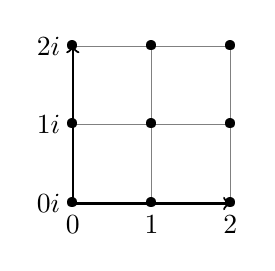
\begin{tikzpicture}
\draw[step=1cm,gray,very thin] (0,0) grid (2,2);
\draw[thick,->] (0,0) -- (2,0);
\draw[thick,->] (0,0) -- (0,2);
\foreach \x in {0,1,2}
   \draw (\x cm,1pt) -- (\x cm,-1pt) node[anchor=north] {$\x$};
\foreach \y in {0,1,2}
    \draw (1pt,\y cm) -- (-1pt,\y cm) node[anchor=east] {$\y i$};
\foreach \Point in {(0,0), (0,1), (0,2), (1,0), (1,1), (1,2), (2,0), (2,1), (2,2)}{
    \node at \Point {\textbullet};
}
\end{tikzpicture}
\end{center}\par 
Voici une grille où chaque point représente un élément de $\C_3$. On voit que les coefficients sont dans $\F_3$ et que le nombre imaginaire $i$ est présent.\par 
Les opérations usuelles ont lieu comme pour $\F_3$. Par exemple, $(2+2i)+(1)=3+2i=2i$. On remarque que l'opération modulo se fait selon un axe. C'est-à-dire que si on "dépasse" 2 horizontalement, on reste sur la même ordonnée, et inversement à la verticale. \par 
Pour la multiplication, il faut faire attention car on prend en compte $i$ tel que $i^2=-1$. Ainsi, $(2+2i)\cdot(2+i)=4+2i+4i+2i^2=4+6i-2=1+1=2$.
\subsection{Représentation}
Comme je l'ai dit plus tôt (ici \ref{Visualisation}), on peut voir les corps finis comme des effets spéciaux. Mais on peut voir ce corps complexe comme un anneau. Imaginons que je prenne le quadrillage vu ce-dessus, et que je colle les deux faces horizontales ensemble. J'obtiens alors un cylindre vide. Si je colle ensuite les deux extrémités de ce tube ensemble, j'ai un anneau. On voit alors que toutes les opérations sont modulaires car on ne peut pas "sortir" de l'anneau.

\subsection{Construction des opposés}
Chaque élément doit avoir son opposé, c'est-à-dire que $\forall x\exists y$ tels que $x+y=0$. Pour chaque élément $a+ib$, son inverse est $(p-a)+(p-b)i$. \par 
Par exemple, l'opposé de $2+i$ est $1+2i$, car $(2+i)+(1+2i)=3+3i=0$. Graphiquement, si on part du point $2+i$, on se déplace une fois à droite, donc on revient à l'abscisse 0, puis on monte deux fois, pour revenir à une ordonnée de 0.

\subsection{Construction des inverses}
La construction des inverses est plus subtile, car on a vu plus haut que ce n'était pas possible pour tous les $p$ premiers. Il faut que $a^2+b^2\neq0\forall a,b\in\F_p$. Dans $\F_3$, c'est bien le cas. On peut alors calculer l'inverse d'un élément de deux manières différentes :
\begin{enumerate}
\item Avec la définition de l'inverse d'un complexe, donc $z^{-1}=\frac{a-ib}{a^2+b^2}$. Si on a une fraction, il faut bien penser à prendre l'inverse selon $\F_p$.
\item En résolvant l'équation $(a+ib)\cdot(c+id)=1\Rightarrow ac+iad+ibc+i^2bd=(ac-bd)+i(ad+bc)=1\Rightarrow ac-bd=1\text{ et }ad+bd=0$
\end{enumerate}

\section{Définition}
On définit le corps $\C_p$ tel que $\C_p = \{a+ib\ |\ a,b\in\F_p\}$. \par 
En réalité, notre corps n'est pas un "corps complexe" mais plutôt une extension quadratique de $\F_p$, c'est-à-dire $\F_{p^2}$, contenant $p^2$ éléments. Cependant, ça reste intéressant, c'est pourquoi j'ai tenu à inclure cette extension.

\end{document}
